% Standalone TSGG pipeline figure — compile: pdflatex tsgg_framework.tex
\documentclass[border=2pt]{standalone}
\usepackage{tikz}
\usetikzlibrary{arrows.meta,positioning,fit}

\begin{document}
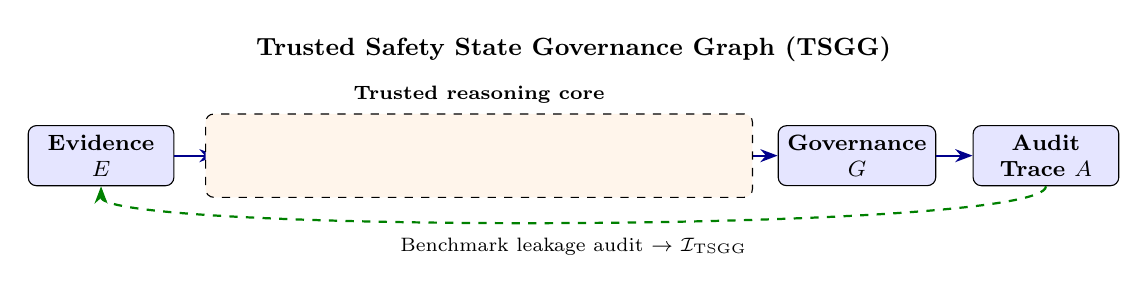
\begin{tikzpicture}[
  stage/.style={draw, rounded corners=3pt, minimum width=1.85cm, minimum height=0.75cm,
                align=center, font=\footnotesize\bfseries, fill=blue!10},
  trust/.style={draw, dashed, rounded corners=3pt, fill=orange!8, inner sep=4pt},
  flow/.style={-{Stealth[length=2.2mm]}, thick, draw=blue!55!black},
  audit/.style={-{Stealth[length=2.2mm]}, thick, draw=green!50!black, dashed},
]

\node[stage] (ev) at (0,0) {Evidence\\$E$};
\node[stage] (ss) at (2.4,0) {Safety\\State $S$};
\node[stage] (ct) at (4.8,0) {Causal\\Transition $C$};
\node[stage] (rec) at (7.2,0) {Recom.\\$R$};
\node[stage] (gov) at (9.6,0) {Governance\\$G$};
\node[stage] (aud) at (12.0,0) {Audit\\Trace $A$};

\foreach \a/\b in {ev/ss, ss/ct, ct/rec, rec/gov, gov/aud} {
  \draw[flow] (\a) -- (\b);
}

\node[trust, fit=(ss) (ct) (rec), label={[font=\scriptsize\bfseries]above:Trusted reasoning core}] {};
\node[font=\scriptsize, align=center] at (6,-1.15)
  {Benchmark leakage audit $\rightarrow$ $\mathcal{I}_{\mathrm{TSGG}}$};

\draw[audit] (aud.south) .. controls +(0,-0.6) and +(0,-0.6) .. (ev.south);

\node[font=\small\bfseries] at (6,1.35) {Trusted Safety State Governance Graph (TSGG)};

\end{tikzpicture}
\end{document}
